% --- LaTeX Homework Template - S. Venkatraman ---

% --- Set document class and font size ---

\documentclass[letterpaper, 12pt]{article}

% --- Package imports ---

\usepackage{
  amsmath, amsthm, amssymb, mathtools, dsfont,	  % Math typesetting
  graphicx, wrapfig, subfig, float,                  % Figures and graphics formatting
  listings, color, inconsolata, pythonhighlight,     % Code formatting
  fancyhdr, sectsty, hyperref, enumerate, enumitem,
  lmodern, textcomp} % Headers/footers, section fonts, links, lists
\usepackage{amscd}
\usepackage{booktabs}
\usepackage{currency}
\usepackage{adjustbox}
\usepackage[title]{appendix}
%\usepackage[
%  format=plain,
%  justification=raggedright,
%  singlelinecheck=false
%]{caption}

%Easy to define your set up with keys
\DefineCurrency{EUR}{
    name={euro},
    plural={euros},
    symbol={\euro},
    iso={EUR},
%   kind=iso, %
    kind=symbol,
%   base=2,
}

% --- Page layout settings ---

% Set page margins
\usepackage[left=2.5cm, right=2.5cm, bottom=1in, top=1.1in, headsep=0.2in]{geometry}

% Anchor footnotes to the bottom of the page
\usepackage[bottom]{footmisc}

% Set line spacing
\renewcommand{\baselinestretch}{1.2}

% Set spacing between paragraphs
\setlength{\parskip}{1.5mm}

% Allow multi-line equations to break onto the next page
\allowdisplaybreaks

% Enumerated lists: make numbers flush left, with parentheses around them
\setlist[enumerate]{wide=0pt, leftmargin=21pt, labelwidth=0pt, align=left}
\setenumerate[1]{label={(\arabic*)}}

% --- Page formatting settings ---

% Set link colors for labeled items (blue) and citations (red)
\hypersetup{colorlinks=true, linkcolor=blue, citecolor=black}


% Make reference section title font smaller
\renewcommand{\refname}{\large\bf{References}}

% --- Settings for printing computer code ---

% Define colors for green text (comments), grey text (line numbers),
% and green frame around code
\definecolor{greenText}{rgb}{0.5, 0.7, 0.5}
\definecolor{greyText}{rgb}{0.5, 0.5, 0.5}
\definecolor{codeFrame}{rgb}{0.5, 0.7, 0.5}

% Define code settings
\lstdefinestyle{code} {
  frame=single, rulecolor=\color{codeFrame},            % Include a green frame around the code
  numbers=left,                                         % Include line numbers
  numbersep=8pt,                                        % Add space between line numbers and frame
  numberstyle=\tiny\color{greyText},                    % Line number font size (tiny) and color (grey)
  commentstyle=\color{greenText},                       % Put comments in green text
  basicstyle=\linespread{1.1}\ttfamily\footnotesize,    % Set code line spacing
  keywordstyle=\ttfamily\footnotesize,                  % No special formatting for keywords
  showstringspaces=false,                               % No marks for spaces
  xleftmargin=1.95em,                                   % Align code frame with main text
  framexleftmargin=1.6em,                               % Extend frame left margin to include line numbers
  breaklines=true,                                      % Wrap long lines of code
  postbreak=\mbox{\textcolor{greenText}{$\hookrightarrow$}\space} % Mark wrapped lines with an arrow
}

% Set all code listings to be styled with the above settings
\lstset{style=code}

% --- Math/Statistics commands ---

% Add a reference number to a single line of a multi-line equation
% Usage: "\numberthis\label{labelNameHere}" in an align or gather environment
\newcommand\numberthis{\addtocounter{equation}{1}\tag{\theequation}}

% Shortcut for bold text in math mode, e.g. $\b{X}$
\let\b\mathbf

% Shortcut for bold Greek letters, e.g. $\bg{\beta}$
\let\bg\boldsymbol

% Shortcut for calligraphic script, e.g. %\mc{M}$
\let\mc\mathcal

% \mathscr{(letter here)} is sometimes used to denote vector spaces
\usepackage[mathscr]{euscript}

% Convergence: right arrow with optional text on top
% E.g. $\converge[w]$ for weak convergence
\newcommand{\converge}[1][]{\xrightarrow{#1}}

% Normal distribution: arguments are the mean and variance
% E.g. $\normal{\mu}{\sigma}$
\newcommand{\normal}[2]{\mathcal{N}\left(#1,#2\right)}

% Uniform distribution: arguments are the left and right endpoints
% E.g. $\unif{0}{1}$
\newcommand{\unif}[2]{\text{Uniform}(#1,#2)}

% Independent and identically distributed random variables
% E.g. $ X_1,...,X_n \iid \normal{0}{1}$
\newcommand{\iid}{\stackrel{\smash{\text{iid}}}{\sim}}

% Equality: equals sign with optional text on top
% E.g. $X \equals[d] Y$ for equality in distribution
\newcommand{\equals}[1][]{\stackrel{\smash{#1}}{=}}

% Math mode symbols for common sets and spaces. Example usage: $\R$
\newcommand{\R}{\mathbb{R}}   % Real numbers
\newcommand{\C}{\mathbb{C}}   % Complex numbers
\newcommand{\Q}{\mathbb{Q}}   % Rational numbers
\newcommand{\Z}{\mathbb{Z}}   % Integers
\newcommand{\N}{\mathbb{N}}   % Natural numbers
\newcommand{\F}{\mathcal{F}}  % Calligraphic F for a sigma algebra
\newcommand{\El}{\mathcal{L}} % Calligraphic L, e.g. for L^p spaces

% Math mode symbols for probability
\newcommand{\pr}{\mathbb{P}}    % Probability measure
\newcommand{\E}{\mathbb{E}}     % Expectation, e.g. $\E(X)$
\newcommand{\var}{\text{Var}}   % Variance, e.g. $\var(X)$
\newcommand{\cov}{\text{Cov}}   % Covariance, e.g. $\cov(X,Y)$
\newcommand{\corr}{\text{Corr}} % Correlation, e.g. $\corr(X,Y)$
\newcommand{\B}{\mathcal{B}}    % Borel sigma-algebra

% Other miscellaneous symbols
\newcommand{\tth}{\text{th}}	% Non-italicized 'th', e.g. $n^\tth$
\newcommand{\Oh}{\mathcal{O}}	% Big-O notation, e.g. $\O(n)$
\newcommand{\1}{\mathds{1}}	% Indicator function, e.g. $\1_A$

% Additional commands for math mode
\DeclareMathOperator{\argmax}{argmax}    % Argmax, e.g. $\argmax_{x\in[0,1]} f(x)$
\DeclareMathOperator{\argmin}{argmin}    % Argmin, e.g. $\argmin_{x\in[0,1]} f(x)$
\DeclareMathOperator{\spann}{Span}       % Span, e.g. $\spann\{X_1,...,X_n\}$
\DeclareMathOperator{\bias}{Bias}        % Bias, e.g. $\bias(\hat\theta)$
\DeclareMathOperator{\ran}{ran}          % Range of an operator, e.g. $\ran(T) 
\DeclareMathOperator{\dv}{d\!}           % Non-italicized 'with respect to', e.g. $\int f(x) \dv x$
\DeclareMathOperator{\diag}{diag}        % Diagonal of a matrix, e.g. $\diag(M)$
\DeclareMathOperator{\trace}{trace}      % Trace of a matrix, e.g. $\trace(M)$

% Numbered theorem, lemma, etc. settings - e.g., a definition, lemma, and theorem appearing in that 
% order in Section 2 will be numbered Definition 2.1, Lemma 2.2, Theorem 2.3. 
% Example usage: \begin{theorem}[Name of theorem] Theorem statement \end{theorem}
\theoremstyle{definition}
\newtheorem{theorem}{Theorem}[section]
\newtheorem{proposition}[theorem]{Proposition}
\newtheorem{lemma}[theorem]{Lemma}
\newtheorem{corollary}[theorem]{Corollary}
\newtheorem{definition}[theorem]{Definition}
\newtheorem{example}[theorem]{Example}
\newtheorem{remark}[theorem]{Remark}

% Un-numbered theorem, lemma, etc. settings
% Example usage: \begin{lemma*}[Name of lemma] Lemma statement \end{lemma*}
\newtheorem{theorem*}{Theorem}
\newtheorem{proposition*}{Proposition}
\newtheorem{lemma*}{Lemma}
\newtheorem{corollary*}{Corollary}
\newtheorem{definition*}{Definition}
\newtheorem{example*}{Example}
\newtheorem{remark*}{Remark}
\newtheorem{claim}{Claim}

% --- Left/right header text (to appear on every page) ---
  
% Include a line underneath the header, no footer line
\pagestyle{fancy}
\renewcommand{\footrulewidth}{0pt}
\renewcommand{\headrulewidth}{0.4pt}

% --- Set path for images ---

\graphicspath{{images/}{../images/}}

% Left header text: course name/assignment number
\lhead{Robinhood Dataset Analysis}

% Right header text: your name
\rhead{Federico Vittorio Cortesi}

% --- Document starts here ---

\begin{document}
\section{Introduction}

In recent years, the rise of commission-free trading platforms has profoundly reshaped retail investor behavior and sparked growing interest among scholars in behavioral finance. 
One of the most prominent examples is Robinhood, a mobile-first brokerage that gained widespread popularity for eliminating trading fees and offering a highly gamified user experience. 
The platform attracted a large number of retail investors, particularly young and inexperienced individuals.
\footnote{According to Robinhood’s IPO filing, the typical user on the platform is 31 years old, with an average account balance of approximately \$3,500. Notably, around half of the platform’s users are investing for the first time.}

An important development in the empirical literature was the release of Robintrack, an open-source dataset that tracks the number of Robinhood users holding individual stocks over time. 
This data, which was collected via Robinhood's public API, provides a rare opportunity to directly observe the trading dynamics and portfolio shifts of real retail investors. 
The dataset can be downloaded from \url{https://robintrack.net/}.

Several recent studies, including \cite{Fedyk2024} and \cite{Welch2022}\footnote{it must be noted that the former explicitly follows the mehtod of the latter}, 
have leveraged the Robintrack dataset to examine retail investor performance. 
Their findings suggest that Robinhood investors—contrary to popular belief—exhibited strong market timing and outperformed passive benchmarks. 
In particular, these papers report significant cumulative returns and positive alpha using standard factor models.

In this paper, we revisit these claims by constructing an alternative methodology for portfolio formation based on the same dataset. 
Specifically, we analyze whether the returns of Robinhood users’ favorite stocks exhibit stochastic dominance over benchmark indices.
Our goal is to offer a more nuanced assessment of whether retail investors truly generate abnormal returns or whether previous results may be driven by sample selection or methodological choices.
\section{Robinhood Dataset}
\subsection{Description of the Dataset}
This data is retrieved from \url{https://robintrack.net/}, the creator retrieved data from the official Robinhood API.

The dataset contains the number of Robinhood users holding at least one share of 8,221 securities. The available data spans from February 5, 2018, to August 13, 2020, covering 818 days (data is available also for non-trading days). Although the data was originally recorded hourly, I aggregated it to a daily frequency by computing the average number of holders per day to simplify computations due to the dataset's size. This aggregation can be easily reversed if needed. 


\begin{figure}[h!]
        \centering
        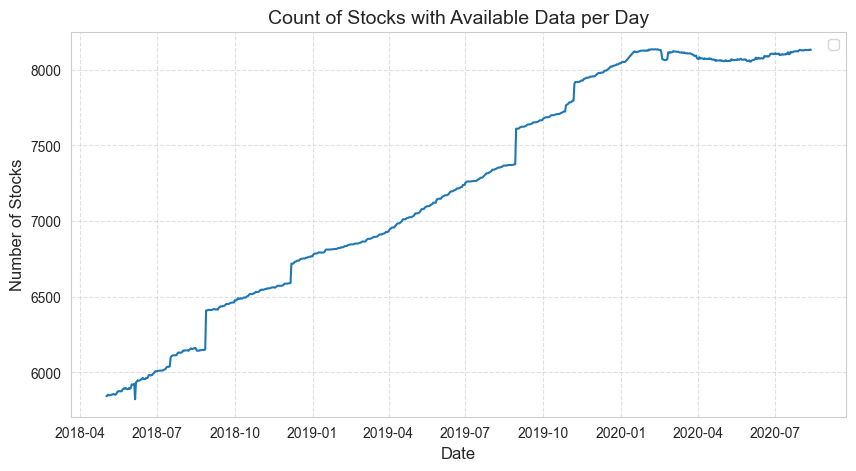
\includegraphics[width=0.8\linewidth]{Images/no_stocks_date.png}
        
\end{figure}


\paragraph{Handling NaNs}  
The original dataset contains missing values for 3,331 securities, primarily in the earlier periods. In some cases, assets appear in the dataset only after a certain date, despite being publicly traded before. It is important to distinguish between missing values and zero values, as they represent different concepts. Some securities exhibit a sudden increase from zero to a larger number of holders, but interpreting these as errors would impose an assumption on investor behavior.  

\noindent Additionally, 1,248 securities have at least one recorded zero in the number of holders. The majority of missing data corresponds to small-cap stocks, which collectively account for at most 3 percent of total market capitalization. Given the limited impact of these securities on overall retail activity, I opted to remove all securities with missing values to ensure consistency in the dataset.  



\subsubsection{Distribution of Key Features (Log-Transformed)}
The distributions of trading volume, market capitalization, and retail holders were initially highly skewed, with a few extreme values dominating the dataset. To address this, I applied a logarithmic transformation: $x^\prime = \log(1+x)$. 

This transformation reduces the impact of outliers, enhances interpretability by making the data more symmetric, and facilitates comparisons between stocks of different sizes.

The key observations after applying the transformation are:
\begin{itemize}
    \item \textbf{Trading Volume:} The distribution appears approximately normal, centered around a peak, with a slight left tail. While most stocks have relatively low trading volume, a few highly traded stocks, such as large-cap or meme stocks, exist but no longer dominate the distribution.
    \item \textbf{Market Capitalization:} The transformed market capitalization data exhibits a bell-shaped curve, suggesting a more balanced spread across small, mid, and large-cap stocks. However, some large-cap stocks remain in the extreme right tail, indicating that a few companies, such as Apple and Microsoft, are significantly larger than the majority.
    
    \item \textbf{Retail Holders:} The number of retail holders follows a roughly log-normal distribution, confirming that a small number of stocks attract massive retail participation while most remain relatively unpopular. The left tail suggests that many stocks have very few retail holders, reinforcing the notion that retail trading is concentrated in a subset of securities.
\end{itemize}

\begin{figure}[h!]
    \centering
    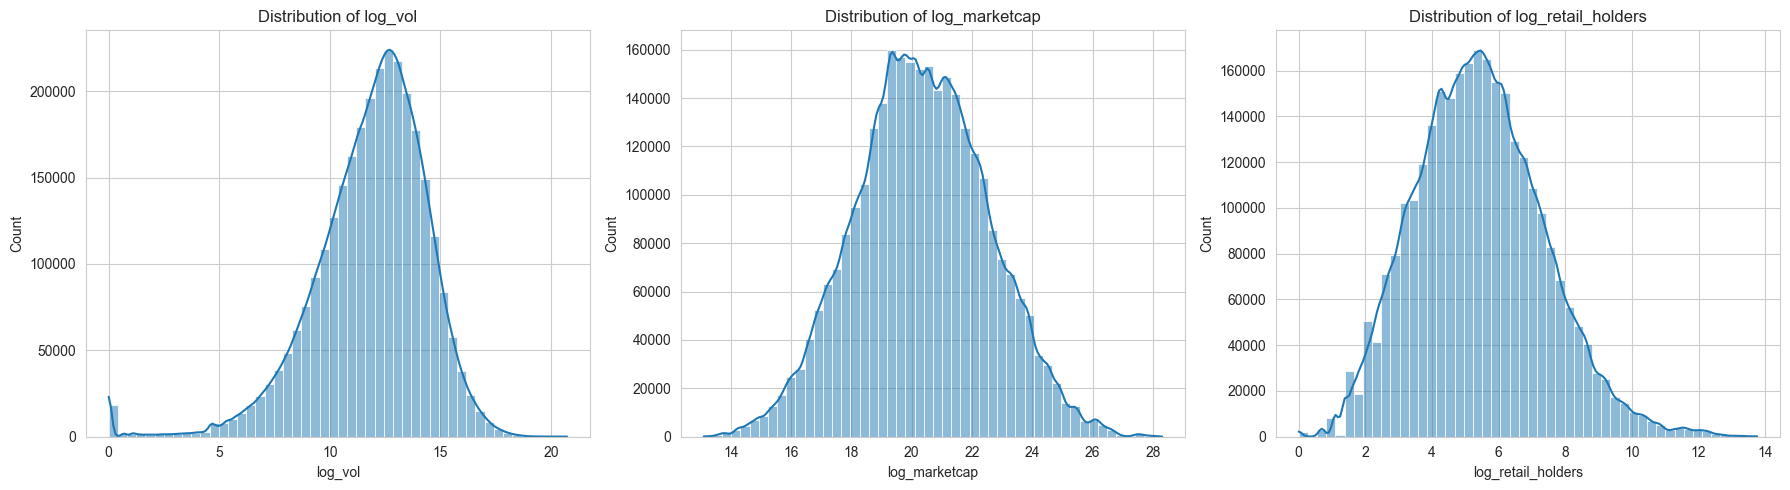
\includegraphics[width=1\linewidth]{Images/Distributions.png}
\end{figure}












\subsection{Comparing the Portfolios}
\subsubsection{Methodology and Overview} 
To build a representative portfolio of the average Robinhood investor, it is necessary to retrieve the prices of the securities. A capitalization-weighted approach can be used, multiplying the price of each security by the number of users who hold it. This approach assumes that all Robinhood users hold a similar number of shares for a given ticker, or that the distribution of shares held per user follows a normal distribution.  

Over the years covered in the dataset, Robinhood has gained a significant number of users. Data on active users is available on Statista\footnote{\url{https://www.statista.com/statistics/822176/number-of-users-robinhood/}}, though only on a yearly basis. Comparing the Statista figures with Robinhood's reported numbers for 2023 suggests that the active user count corresponds to December 31 of each year. This data could later be used to normalize the number of users and build a reference portfolio.  

The total number of open positions can be computed as the sum of all investors who hold at least one security in each asset, effectively a row-wise sum of the dataset.  

Market data for all securities was retrieved from the CRSP\footnote{The Center for Research in Security Prices, based at the University of Chicago, provides high-quality historical market data widely used in finance research and investment analysis.} database, accessed via WRDS. However, only 8,099 securities are available in CRSP, as it focuses exclusively on American assets. The difference in open positions between the full dataset and the CRSP subset is minimal. If, instead, all securities with missing values are dropped, leaving only 5,221 securities, the gap widens.

\begin{figure}[h!]
        \centering
        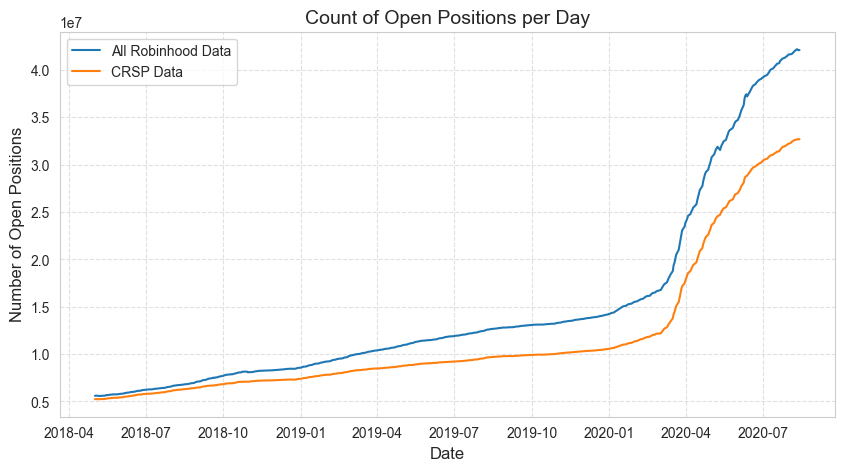
\includegraphics[width=0.8\linewidth]{Images/no_positions_vs_date_drop.png}
\end{figure}

The graph illustrates the  count of open positions per day  on Robinhood from April 2018 to mid-2020, showing a  steady increase  over time, with a  sharp acceleration in early 2020. This surge aligns with the onset of the  COVID-19 pandemic, which likely drove a significant influx of new retail investors seeking market opportunities amid economic uncertainty and stimulus checks. 



\subsubsection{Retail Investors Prefer "Famous" Stocks}

The majority of the securities are common shares, representing about 57.9\%. ETFs represent about 23.7\% and other funds are the 9.2\% of the dataset. Other structured investments, REITs, and ADRs cover the remaining part.

Analysing the securities by market capitalisation about 82.9\% is represented by stocks and 9.6\% by ETFs. If we look at the "Retail Market Cap" (i.e. number of positions times price), 89.2\% of securities are stocks and 5.8\% are ETFs.  

Looking at the securities Robinhood users prefer holding, ranked by "Retail Market Cap", investors prefer holding smaller cap stock. A qualitative analysis shows "famous" stocks, such as Tesla, Starbucks, and Nvidia to name a few, to appear among the most popularly owned.

\subsubsection{Possible Measures of Divergence} 
\paragraph{Rank Distance} 
To describe the preference of retail investors for smaller cap stock I propose the following measure:
\begin{align*}
    d_R = \sum_{i=1}^N \frac{R^{\text{Mkt}}_i-R^{\text{RH}}_i}{R^{\text{RH}}_i}
\end{align*}
Where $R^{\text{Mkt}}_i$ is the rank of the $i^\text{th}$ security by market cap, and $R^{\text{RH}}_i$ is the rank by retail market cap. The normalization by $R^{\text{RH}}_i$ reduces the impact of small-cap stocks with minor ranking differences.

\begin{figure}[h]
        \centering
        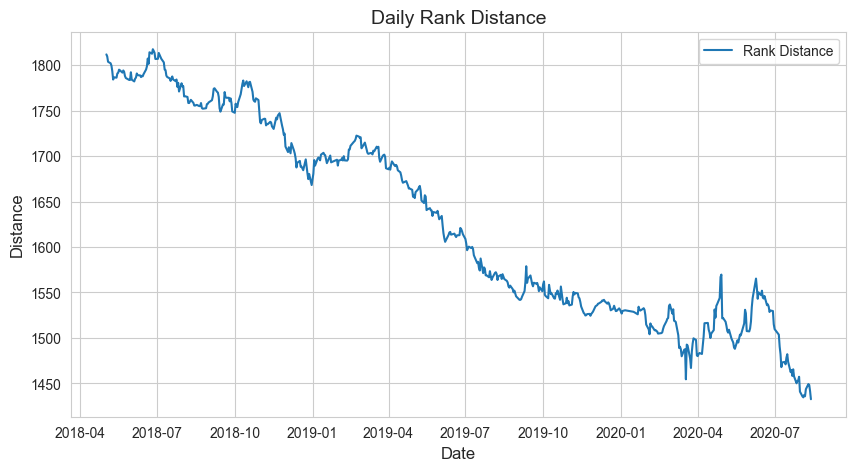
\includegraphics[width=0.8\linewidth]{Images/rank_distance.png}
\end{figure}

The plotted Daily Rank Distance suggests a clear downward trend from early 2018 to mid-2020, indicating that the ranking of stocks by retail market cap has become increasingly aligned with the ranking by total market cap. Initially, the distance is above 1800, gradually declining towards 1450. This implies that retail investors, who originally exhibited a stronger preference for smaller-cap stocks, have progressively shifted towards stocks that are more representative of the broader market.

Between 2018 and 2019, the decline is relatively steady, reflecting a gradual change in retail investment behavior. However, the trend accelerates in 2019 and 2020, suggesting a more pronounced shift. The beginning of 2020 shows increased volatility, with occasional upward spikes, which could be attributed to market disruptions, possibly linked to the COVID-19 crash and the subsequent retail trading boom. The rapid expansion of retail investing during this period, fueled by stimulus checks and zero-commission trading, may have led to temporary deviations, but the overall trend continues downward.

A sustained decrease in rank distance suggests that retail investors have moved closer to institutional preferences, potentially increasing their exposure to large-cap stocks or index-tracking assets. If this trend persists, it would indicate a continued assimilation of retail behavior into the broader market structure. Conversely, a reversal in this pattern could signal renewed speculative activity or a shift back to small-cap stocks.

\section{Building the Robinhood Portfolio}
\subsection{Methodology}
\subsubsection{Weights Methods} 
\cite{Fedyk2024} and \cite{Welch2022} use the same approach to build the performance of the Robinhood crowd (or "reference index"): 
they build daily weights and then apply the weights from the previous day to daily stock returns, directly building portfolio returns. 

First, it is necessary to define how those weights are computed. They define two different types of weights, although they yield similar findings in their analysis.

The first method is the "dollar method", which assumes that every investor represents an equal dollar amount investment in the stock. 
\begin{equation}
    w^{\text{dollar}}_{i,t} = \frac{N_{i,t}}{\sum_j N_{j,t}}
\end{equation}

where $w_{i,t}$ is the Robinhood portfolio weight of security $i$ at time $t$ and $N_{i,t}$ is the number of investors in security $i$ at time $t$.

Alternatively, they define the "share method", where each Robinhood investor in a stock represents a one share investment in that stock.
\begin{equation}
    w^{\text{share}}_{i,t} = \frac{N_{i,t}\cdot P_{i,t}}{\sum_j N_{j,t}\cdot P_{j,t}}
\end{equation}
where $P_{j,t}$ is the price of stock $j$ at time $t$.

\subsubsection{Different Approaches to Compute Performance}
As explained above, the biggest limitation of the Robintrack dataset is that it counts the number of users holding a certain security and doesn't provide any information on the amount invested in a particular security. 

The other authors build the portfolio returns by multiplying weights by their daily returns\footnote{returns are computed directly by CRSP and are adjusted for dividends, e.g. if $P_0=10$ and $D_1=5$ and $P_1=5$ returns would be 0\%}, 
assuming that the weights, however computed, represent a certain share of wealth in a stock of the Robinhood crowd.
\begin{equation}
    r_{RH,t} = \sum_{i=1}^N w_{i,t}\cdot r_{i,t}
\end{equation}

On the other hand, I tried to compute the value of the Robinhood portfolio by doing a weighted sum of the prices of the securities in the dataset.
Conceptually, this represents the portfolio of an investor who decides to allocate a certain number (or percentage) of shares to each security.
I will call this the "Price" method, or simply my method.

We can therefore define the value of the Robinhood Portfolio as follows:
\begin{equation}
    V_{RH,t}=\sum_{i=1}^N w^{\text{dollar}}_{i,t}\cdot P_{i,t}
\end{equation}

Returns are then computed from the value of the overall portfolio as:
\begin{equation}
    r_{RH,t} = \ln\left(\frac{V_{RH,t}}{V_{RH,t-1}}\right)
\label{returns_mine}
\end{equation}

In this paper I prefer using log-returns where possible. 

\subsubsection{Capturing the Persistence of Investor Composition}
Although both approaches ultimately yield a time series of Robinhood portfolio returns, there is a fundamental difference in what these return paths represent.

In the method used by \cite{Fedyk2024} and \cite{Welch2022}, the portfolio is effectively rebalanced every day to reflect the current composition of investor popularity.
Each day's return is computed based on that day's weights and the corresponding daily stock-level returns.
This provides a valid snapshot of the average return generated by the stocks held on a given day.

However, this approach does not preserve the economic exposure that investors accumulate through time.
A stock that was extremely popular for several days but declines in popularity just before a price spike will have minimal influence on the portfolio's return when that spike occurs.
Only the weights at time $t-1$ affect the return at time $t$\footnote{Previous day's weights are taken to prevent look-ahead bias}, so the model captures immediate sentiment shifts but not the cumulative effects of holding positions over time.

In contrast, the methodology I propose (\ref{returns_mine}) applies weights to stock prices and computes returns from changes in total portfolio value.
This implies that a stock that was heavily weighted yesterday continues to influence portfolio performance today, even if its popularity has declined.
The return reflects both the dynamics of price changes and the path dependency of investor composition.

As a result, my method embeds the effects of investor flows, popularity shifts, and concentration in the actual evolution of portfolio value.
The cumulative performance is not a sequence of disconnected daily snapshots, but a reflection of how crowd behavior builds, persists, and unwinds over time.

Conceptually, this distinction is important when studying behavioral dynamics.
Retail investor behavior—particularly on platforms like Robinhood—is driven not only by cross-sectional preferences at a point in time but also by persistent patterns of attention, sentiment, and herding.
A portfolio that evolves with these behavioral shifts provides a more realistic measure of the actual wealth path experienced by retail investors, rather than an idealized, continually rebalanced index.

In this sense, computing returns from the portfolio value offers a more structurally consistent and behaviorally meaningful representation of the Robinhood crowd's investment trajectory.


\section{Comparing Returns and Risk measures}
The biggest difference do not appear when using different kinds of weights ("dollar" or "share" method) but rather when building the portfolio from prices or returns. 
Moreover, Fedyk and Welch build their portfolio only using common american stocks (share code 10 or 11). 
In my final analysis I look at all types of securities but significant differences emerge even when using the same sample. 
Additionally, by recreating their method employed by the other authors we can analyse its return when dealing with all kinds of securities. 
In section \ref{diff_samples} I compare returns using only common stocks or the full sample of securities, in the other sections of this paper I will use the full sample unless explicitly stated.

As the other authors have claimed in their papers, the Portfolio built directly from returns had a significantly higher cumulative return compared to the market and positive alpha.

I will proceed to analyse in more detail the distribution of returns of different Robinhood portfolios, showing that my method depicts a far less rosy picture of the "Robinhood strategy".

Moreover, \cite{Fedyk2024} has analysed extensively the differences between the portfolio obtained using the share method and the dollar method. 
We'll focus on the dollar method since it is the same approach I use to compute weights.

\subsection{Constructing Moving Averages}
I begin by computing daily log returns as $r = \ln\left(\frac{P_1}{P_0}\right)$, knowing that for small $x$, $\ln(1+x)\approx x$. 
Defining log returns allows us to simply compute moving averages, showing the profitability of the Robinhood portfolio at different time frames.
Conceptually, the value of an $n$-day moving average on a given date $T$ represents the return an investor would have earned by initiating the position at the open of day $T-n$ and holding it continuously up to close of day $T$.
More rigorously, for a given horizon of $n$ days:
\begin{equation}
    r_n = \sum_{t=T-n+1}^{T} r_t \approx \ln \left( \prod_{t=T-n+1}^{T} (1+R_t) \right)
\end{equation}
where $r_t$ are dauly log returns and $R_t$ are daily percentage returns.


\subsection{Retail Performance Under Different Samples}\label{diff_samples}




\subsubsection{Rolling Returns Across Investment Horizons}
\paragraph{Common Stocks Only}
At short horizons (5–30 days), the two Robinhood portfolios (Fedyk and Mine) display highly similar dynamics, with both closely tracking market indices and exhibiting bursts of volatility during periods of market stress, particularly around the onset of the COVID-19 crash. 
This suggests that in the very short term, retail investors tend to move in tandem with broader market trends, with limited divergence in return profiles across methodologies.
However, at the 120-day horizon, both Robinhood portfolios outperform the S\&P 500 and a World ETF\footnote{I've used Vanguard's VOO for the S\&P500 and Vanguard's VT as a World Equity ETF}. 

This finding is consistent with the idea that many retail investors, especially on Robinhood, engaged in "buy-the-dip" behavior during the COVID-19 crash. 
Their increased exposure to beaten-down or speculative stocks during the downturn appears to have been rewarded in the subsequent rebound. 
Importantly, this also coincides with a period of explosive growth for the platform itself, which may have amplified attention and capital inflows into popular names.

Nonetheless, this post-crash outperformance comes after a prolonged period of clear underperformance. 
Prior to March 2020, both Robinhood portfolios consistently lag behind the benchmark indices, with my method in particular reflecting substantial drawdowns and poor stock selection.

What differentiates the two methods most clearly is the strength of the post-COVID recovery. 
While Fedyk’s method shows a relatively steady climb, my price-based approach rebounds even more sharply after March 2020. 
This reflects the fact that, under my methodology, investor positions are not rebalanced away from prior favorites. 
As a result, stocks that surged after the crash contributed disproportionately to the portfolio’s recovery. 

In sum, the 120-day results provide two key insights: first, that retail traders on Robinhood did benefit from post-crisis market dynamics, and second, that the magnitude and nature of this benefit depends heavily on the modeling approach, particularly when capturing persistence in portfolio composition.

\begin{figure}[h!]
    \centering
    \includegraphics[width=1\linewidth]
    {../images/returns/comparison_1.png}
\end{figure}

\paragraph{Full Universe of Securities}

We now extend the analysis to all securities in the dataset, including ETFs, REITs, and structured products.

Expanding the sample, we still observe that short-term movements (5–30 days) remain closely correlated across all portfolios, with limited divergence in returns or volatility between methods.

However, the performance gap widens at longer horizons. 
In contrast to the stock-only case, where both Robinhood portfolios outperform after the crash, here the drawdowns, particularly in the price-based portfolio, are deeper and more persistent.

Low performance spans the entire pre-COVID period: my portfolio underperforms continuously throughout 2019, while Fedyk’s stays closer to the benchmarks but still lags in absolute terms.

At the 563-day horizon, both Robinhood portfolios end below the S\&P 500 and the World ETF.
My portfolio, while showing a stronger post-crash rebound, barely catches up to the S\&P 500 by the end of the sample, and only due to its heavier exposure to post-crash winners.
Fedyk’s method performs slightly better but remains clearly below the benchmark, reversing the apparent outperformance seen in the stock-only sample.

\begin{figure}[h!]
    \centering
    \includegraphics[width=1\linewidth]
    {../images/returns/comparison_2.png}
\end{figure}

A detailed description of the distributions can be found in table \ref{tab:returns_all}.

\subsubsection{Distribuional insights}
\paragraph{Common Stocks Only}

The distribution of returns across horizons provides further evidence on the differences between the Robinhood portfolios and the benchmarks.

At short horizons (5–30 days), all portfolios are tightly centered around zero, with relatively similar dispersion. 
Both Robinhood portfolios display slightly higher volatility than the S\&P 500 and the World ETF, with standard deviations of approximately 0.045 for five-day returns, compared to about 0.03 for the benchmarks. 
However, mean returns remain close to zero for all portfolios, and short-term behavior shows limited divergence across methods.

At the 120-day horizon, differences become more evident. 
While Fedyk's portfolio maintains a positive mean log return of approximately 0.05, my price-based portfolio exhibits a negative mean return of about -0.06. 
The median is also much worse, at about -0.14 versus -0.02.
This shift is reflected in the distribution shapes, with my portfolio showing a wider left tail and greater dispersion relative to both Fedyk’s method and the benchmarks.

At the 563-day horizon, the gap further widens. 
The price-based portfolio remains centered around negative returns, with a mean log return of approximately -0.04, while the rebalanced portfolio achieves a positive mean return of 0.17. 
In contrast, the S\&P 500 maintains a strong positive outcome, with a mean log return close to 0.1. 

Despite the strong rebound observed after the COVID-19 crash, the cumulative performance of the price-based portfolio remains significantly weaker, often with higher standard deviation.

\begin{figure}[h!]
    \centering
    \includegraphics[width=1\linewidth]
    {../images/distributions/comparison_1.png}
\end{figure}


A detailed description of the distributions can be found in table \ref{tab:returns_stocks}.

\paragraph{Full Universe of Securities}

Expanding the analysis to include all types of securities slightly alters the distributional patterns compared to the stock-only case.

At short horizons (5–30 days), return distributions remain centered around zero and maintain a similar dispersion across all portfolios. 
Standard deviations are comparable to the stock-only case, around 0.02 for both Robinhood portfolios at the daily level and 0.04 for five-day returns. 
Mean returns are very close to zero, confirming that short-term dynamics are largely unaffected by the broader sample.

At the 120-day horizon, however, differences become more evident. 
Both Robinhood portfolios exhibit flatter distributions with thicker left tails compared to the benchmarks. 
In particular, my price-based portfolio records a negative mean log return of approximately -0.07, while Fedyk’s method also turns slightly negative at around -0.004, unlike in the stock-only case where it remained positive. 
The S\&P 500 maintains a positive mean return over the same horizon, reinforcing the relative weakness of retail portfolios when more asset types are included.

At the cumulative horizon, the gap becomes substantial. My portfolio shows a strongly left-skewed distribution with a mean log return of approximately -0.10.
Fedyk’s portfolio, although positive at around 0.087, remains below the S\&P 500, which achieves a mean return close to 0.1. 
The World ETF again displays lower returns, in line with its broader exposure to international markets.
\begin{figure}[h!]
    \centering
    \includegraphics[width=1\linewidth]
    {../images/distributions/comparison_2.png}
\end{figure}

Descriptive statistics supporting these findings are reported in Table \ref{tab:returns_all}.

\subsection{Analysis of Short-Term Returns and the Impact of COVID}
Comparing the daily returns for the whole period available we can already observe distinct behavior in terms of returns and distributions for the market and Robinhood indeces.
To test whether there are statistically significant differences beteen the mean daily returns of the Robinhood portfolios, the S\&P 500 and the world ETF, I conduct an ANOVA test.
The null hypothesis is that all portfolios have equal mean daily returns.

\subsubsection{Covering the Whole Period}
As expected from the results regarding the cumulative returns, mean daily returns are very similar for the Robinhood Portfolios.
Fedyk's method has a mean of 0.000555, while the method based on prices has a mean of 0.000450.
The ANOVA analysis conducted on these two portfolios, equal to a t-test in this case, has a p-value of 0.9273.
This suggests that at the daily frequency the expected growth rate, i.e. the mean log returns, of the Robinhood portfolios are not statistically different.


In terms of standard deviation, the Robinhood portfolios have relatively larger values, around 0.02, while the market indeces hvae values around 0.15. 
This is consistent with what can be seen from the distributions: retail portfolios have fatter tails while modal returns appear similar across all timeseries.

Conducting ANOVA tests on all possible combinations of these four timeseries, none has an acceptable p-value, results are in table \ref{tab:anova_all}.
However, conducting a Fligner test to assess difference in variances, the Robinhood portfolios show statistically significant differet variances than the market proxies, results are in table \ref{tab:fligner_all}.


Here below the plots of the distributions, while the returns are in table \ref{tab:returns_all}:
\begin{figure}[h!]
    \centering
    
\includegraphics[width=1\linewidth]
    {../images/distributions/st_all.png}
\end{figure}


\subsubsection{Excluding COVID}
This results on daily returns, however, are probably impacted by the noise of the March 2020 crash. 
I run the same analysis filtering the dataframe up to February 3rd 2020, the date in which the pandemic was declared in the US.

In this case point estimates for means differ greatly even among Robinhood Portfolios, with the price based approach yielding -0.000328 on average versus Fedyk's 0.000246.
Nonetheless, also at this level returns are not statistically significant, results can be found in table \ref{tab:anova_before}.

In terms of standard deviation, the market indices show again clearly a different distribution, with variances being markably lower. 
This is corroborated by fligner tests, available in table \ref{tab:fligner_before}.

Here below the plots of the distributions, while the returns are in table \ref{tab:returns_st_before}:
\begin{figure}[H]
    \centering
    
\includegraphics[width=1\linewidth]
    {../images/distributions/st_before.png}
\end{figure}

\subsection{Comments}
Daily returns show a deceptively optimistic view, with the different series having statistically equal log-returns.
However, the retail portfolios carry systematically higher day-to-day risk, amd this compounds as underperformance at the cumulative level before the pandemic.

A one-way ANOVA on daily log returns fails to reject equality of means for any group of series, both including and excluding the pandemic. 

However, looking at the risk dimension, stand deviations differ sharply. 
Fligner-Killeen tests reject homogeneity at any $\alpha$ level whenever a retail series is compared with a market proxy.
As highlighted earlier, this can be easily seen from the shape of the distributions, with correspondingly fatter tails.
In log space, larger dispersion automatically lowers long-run growth because every large swing pulls the cumulative sum away from the average trend.
In other words, retail investors accept more noise than the market but earn no meaurable extra drift in a single day.

Although ANOVA cannot reject equality between the Robinhood portfolios, the point estimates themselves are not identical (compare table \ref{tab:returns_st_before}).
The gap in their mean returns, about -0.0006 log points, rapidly cumulates to -0.25 log points. 
The test lacks power because daily $@s$ is large; the economic impact measured in compounding is evident.

Path dependence widens the difference.
The price-weighted series \ref{returns_mine} embeds a negative correlation between returns and remaining capital.
When a stock falls, its contribution to the portfolio value shrinks, and therefore any subsequent rebound is applied to less capital, exactly how a normal portfolio would work. 
The return-weighted construction re-anchors weights every market close and therefore avoids this drag.
Losses in early 2019 thus penalise the price-weighted portfolio twice.  





%% -------------------------------------------------------------------- %%
%\subsubsection{old}
%
%We can start by loo
%
%
%
%At short-term horizons (5 to 15 days), all three portfolios show similar patterns, with relatively mild fluctuations. Retail returns exhibit slightly higher volatility, particularly for the Robinhood portfolio, indicating that retail investors are more reactive to short-term market movements. The returns across these horizons reflect a degree of correlation, suggesting that, over short periods, retail investors' behavior mirrors that of the broader market, albeit with more pronounced movements.
%
%At the 30- and 60-day horizons, divergence becomes more apparent. The Robinhood portfolio shows a higher degree of volatility, with both larger peaks and deeper troughs compared to the market and the ETF benchmarks (VOO and VT). This volatility suggests that retail traders may be engaging in more speculative behavior or reacting strongly to market news, which could lead to exaggerated responses and momentum chasing. Notably, during periods of rapid market movements (e.g., mid-2020), the Robinhood portfolio experiences sharp rallies, likely driven by retail investor participation in tech stocks or speculative assets.
%
%At the 120-day horizon, the Robinhood portfolio begins to underperform relative to both VOO and VT, particularly in major market downturns like the COVID-19 crash. The underperformance during these periods is consistent with the behavior observed in retail investors during market corrections—often driven by overreaction or poor risk management. However, after the COVID market crash, the Robinhood portfolio shows notable recovery, achieving higher returns than VOO and VT, reflecting retail traders' ability to capitalize on post-crash rebounds, potentially due to increased exposure to riskier assets.
%
%At the 564-day horizon, the long-term performance diverges significantly. The Robinhood portfolio initially lags behind both VOO and the market, reflecting a less optimal asset allocation or suboptimal stock selection. While there is some recovery post-COVID, retail investors still fail to capture the consistent growth observed in the broader market over a longer timeframe. This highlights the challenges that retail investors may face in achieving long-term growth, especially when influenced by short-term market sentiment or reacting to news-driven volatility. Nonetheless, the post-crash rally showcases the potential for retail portfolios to outperform during certain market phases, albeit with higher risk.
%
%Overall, the plot demonstrates that while retail portfolios can experience significant short-term gains, their performance is often more volatile and less consistent over the medium to long term, with periods of underperformance and delayed recoveries.
%
%Looking at the distribution of returns for the same periods other insights can be drawn (compare \ref{tab:returns_stats}). 
%
%
%At shorter horizons (5 to 30 days), the return distributions for all portfolios- market, Robinhood (RH), VOO, and VT- are quite similar, with tightly clustered and symmetric shapes. However, the Robinhood distribution exhibits slightly fatter tails compared to VOO and the market, suggesting that retail investors, particularly those in the Robinhood portfolio, experience more extreme short-term gains and losses. This indicates higher short-term volatility and sensitivity to market movements.
%
%As the horizon increases (60 to 564 days), the Robinhood distribution becomes increasingly dispersed, with wider tails and lower peaks. This shift indicates that retail investors are exposed to higher volatility over longer periods, with greater potential for both positive and negative extreme outcomes. In contrast, VOO and the market distributions remain relatively stable, with tighter and more concentrated peaks. These distributions suggest that diversified portfolios, like VOO and the market index, provide more consistent and lower-risk returns over time.
%
%At the longest horizon (564 days), the Robinhood distribution shows a noticeable left skew, indicating that the portfolio underperforms over the long term. This is consistent with earlier findings of long-term underperformance, where retail investors fail to capture consistent gains in the broader market. In contrast, the VOO distribution is shifted rightward, reflecting stronger and more consistent long-term performance, which is typical of diversified, lower-risk portfolios.
%
%In summary, these distribution plots highlight the increased volatility and higher risk exposure associated with the Robinhood portfolio, especially as the time horizon lengthens. Over both medium and long horizons, retail portfolios are more prone to extreme outcomes, with consistent underperformance relative to the more diversified VOO and market portfolios. This reinforces the conclusion that retail investors, while potentially benefiting from short-term rallies, struggle to maintain consistent returns in the long run due to greater sensitivity to market fluctuations and suboptimal asset selection.
%\paragraph{What Happened during the Pandemic?} Analyzing the same indices from February 3rd, 2020 we can find some relevant insights. 
%
%
%At very short horizons (1-5 days), performance across all portfolios is similar and volatile, with no consistent pattern. However, from the 15-day horizon onward, a clear divergence emerges: Robinhood portfolio returns (orange) begin to outpace both the market indices, which have a high degree of correlation.
%
%This trend becomes particularly evident at 30, 60, and 135-day horizons, where the Robinhood portfolio exhibits significantly higher cumulative gains after a more sluggish start. 
%In contrast, VOO and the market index recover more gradually, with smoother return paths and lower cumulative gains. This reflects broader diversification and reduced exposure to speculative stocks.
%
%We can look at the distributions of returns for this timeframe as well:
%
%
%\subsection{Analysis of Short-Term Market Movements and Volatility, Including the Impact of COVID}
%
%\subsubsection{Return Characteristics and Volatility Analysis}
%\paragraph{including COVID}
%Comparing the daily and 5-day moving average returns for the whole period available we observe really similar behavior in terms of returns and distributions for the marker indices,
%while RH has significantly fatter tails (which can be observed also in the CDF plot).
%
%RH has slightly higher average returns compared to the market (MC) both for 1-day and 5-day returns. For 1-day returns, RH has an average return of 0.000719, which is higher than the market's 0.000396. 
%Similarly, for 5-day returns, RH's average is 0.003281, which is again  higher than the market's 0.001913. 
%In terms of standard deviation, RH shows more volatility in both horizons. 
%The 1-day standard deviation for RH is 0.018809, compared to the market's 0.01547, and for the 5-day returns, RH's standard deviation is 0.041909, while the market's is 0.031198. 
%Therefore, RH consistently exhibits higher returns and higher volatility over both timeframes compared to the market. Detailed distribution are in table \ref{tab:st_returns_stats_all}.
%
%Here below the plots of the time series:
%
%
%\paragraph{Before COVID}
%Excluding returns from February 3rd 2020 might help to reduce some of the noise in the sample and allow us to understand more significant trends about RH investors.
%
%For 1-day returns, RH still has lower average returns compared to the market (MC). 
%RH has an average return of 0.000115, while the market's average is 0.000419.
%
%For the 5-day returns, RH's average is much smaller than that of the market. 
%RH has an average return of 0.000259, while the market's average is 0.002091. 
%
%In terms of standard deviation, RH still exhibits more volatility than the market, but the gap is again smaller than the previous data.
%The 1-day standard deviation for RH is 0.013490, compared to 0.008745 for the market, which shows more volatility for RH but with a smaller gap compared to the earlier dataset where RH had much higher volatility.
%For the 5-day standard deviation, RH has 0.026549, compared to 0.019395 for the market. The difference is still significant, but once again, smaller than the previous dataset where RH showed greater variability.
%
%In conclusion, while RH still exhibits more volatility than the market across both horizons, it now shows lower returns than the market for both 1-day and 5-day periods, possibly due to a more consistent left tail.
%Detailed distribution are in table \ref{tab:st_returns_stats_before}.
%
%Here below the plots of the CDFs and PDFs, both including and exluding covid:
%
%
%\subsubsection{Comments}
%
%The short-term return distribution for the RH portfolio is noticeably "flatter" (higher variance/dispersion) compared to broad market benchmarks like VOO or VT. 
%This is consistent with the "buy-the-dip" behavior highlighted by \cite{Fedyk2024} and \cite{Ardia2023Fast}. 
%Actively buying stocks after extreme negative returns means engaging with assets currently experiencing heightened volatility. Even if the average next-day return was positive during the sample period (as Fedyk found for 1-day holds), 
%the range of potential outcomes for these stressed stocks is much wider than for the diversified market, contributing to the fatter tails and lower peak in the distribution.
%
%    
%A primary driver of the flatter distribution is likely the significant lack of diversification among individual Robinhood investors. As noted by \cite{Fedyk2024} and \cite{Welch2022}, the average user held very few stocks ($\sim\,3$)\footnote{They reach this measure by dividing the estimated number of active users mid august 2020 by the number of open positions, (Section 2.4)}. 
%Individual, concentrated portfolios inherently carry high idiosyncratic risk, leading to much greater return variance compared to diversified market indices represented by VOO/VT.
%    
%Stock selection tilts further contribute to the higher volatility. \cite{Welch2022} found RH investors favoured high-volume stocks, which could be associated with higher attention and volatility. 
%\cite{Fedyk2024} also found no strong evidence of aversion to idiosyncratic volatility. Additionally, \cite{Ardia2023Fast} noted stronger reactions in specific sectors like energy. These preferences likely result in a basket of holdings that is intrinsically more volatile than the overall market.
%
%
\section{Assessing Risk Preferences: A Dual-Criterion Approach}
\subsection{Setup and Definitions}
The results of section \ref{return_section} paint very different pictures of retail investors. 
Using the method set forth by \cite{Welch2022} and \cite{Fedyk2024}, analyzed also in section \ref{fedyk_paper_returns}, yields superior returns and similar drawdowns to the market.
They also conclude that the Robinhood crowd has achieved positive alpha when analyzed under different factor models (table VII, IX, X in \cite{Welch2022} and table 16 in \cite{Fedyk2024}). 
These results appear to be in contrast with the existing literature on retail investing, most notably \cite{BarberOdean2000}.

A more fundamental question, however, is whether those returns are attractive once investors' attitudes toward risk are taken into account.
This section evaluates the Robinhood portfolio against its market benchmarks using two complementary criteria.

First, I adopt the constant-relative-risk-aversion (CRRA) framework, in line with the majority of asset pricing work.
\begin{equation}
    U(W) = 
    \begin{cases}
    \frac{W^{1-\gamma}-1}{1-\gamma}, \gamma\neq 1\\
    \ln(W), \gamma = 1
    \end{cases}
    \label{CRRA}
\end{equation}

By computing the expected utility of both the Robinhood and benchmark portfolios over a grid of possible risk aversion ($\gamma$) values,
I identify the cutoff $\gamma^*$ such that a representative CRRA investor is indifferent between the two.
This delivers a concise, parametric summary of how risk preferences may shape portfolio choice.

Then, I estimate the welfare loss derived from investing in the Robinhood portfolio rather than (i)  not investing or (ii) investing in the market portfolio.
By comparing the certainty-equivalent wealth under each strategy for a CRRA investor, with risk aversion calibrated inside a feasible range,
I obtain dollar-denominated welfare losses that capture the risk-return profile taken by Robinhood investors.

However, this method cannot deliver precise estimates given the limited sample size. 
I therefore employ another method to estimate the risk aversion $\gamma$ from the percentage of wealth invested in the risky asset ($\alpha$), 
precise numbers about the wealth of Robinhood investors are not available, I therefore plot the implied risk aversion over a grid $\alpha$ and compare it to alternative portfolios.

\subsection{Expected Utility and Cutoff}
\subsubsection{Sampling Variability and Finite-Sample Limitations}
Identifying a cutoff level of risk aversion provides a clear criterion for the CRRA utility-maximizing investor: 
it is the minimum $\gamma$ at which an alternative strategy becomes preferred to the Robinhood portfolio.
However, the limited size and noise of the sample imply wide conference intervals for the estimated expected utilities at different $\gamma$ levels.
In practice, this remains a useful conceptual framework to understand how risk preference and beliefs may affect portfolio choice, but in limited samples, its numerical outputs are more illustrative than definitive.
However, this method yields precise results in a very specific case I will describe later. 

Formally, we want to find $\gamma^*$ defined as:
\begin{equation}
    \gamma^* = \min\left\{ \gamma_j : \mathbb{E}[U_p(\gamma_j)] \leq \mathbb{E}[U_m(\gamma_j)] \right\}
    \label{gamma_cutoff}
\end{equation}
where $U_p(\cdot)$ is the utility of the Robinhood portfolio, while $U_m(\cdot)$ is the utility of the market portfolio.

In practice, we apply CRRA utility function (\ref{CRRA}) to each gross return observation and then takes the sample average.
The resulting mean serves as the expected utility implied by the investor's revealed choices over the sample period.
Wealth at time $t$ is equal to gross returns, assuming the initial wealth $W$ to be equal to one without loss of generality.


The main problem related to this approach is inherent to the sample we apply it to, having only 539 observations and inclusion of extreme events such as the COVID crash. 
These factors inflate the sample variability of our mean-utility estimates, so much that regardless of whether we use daily returns, various rolling-window horizons, or subperiods, the resulting confidence intervals remain prohibitively wide.
Figure \ref{fig:cutoff} illustrates this well: 
\begin{figure}[H]
    \centering
    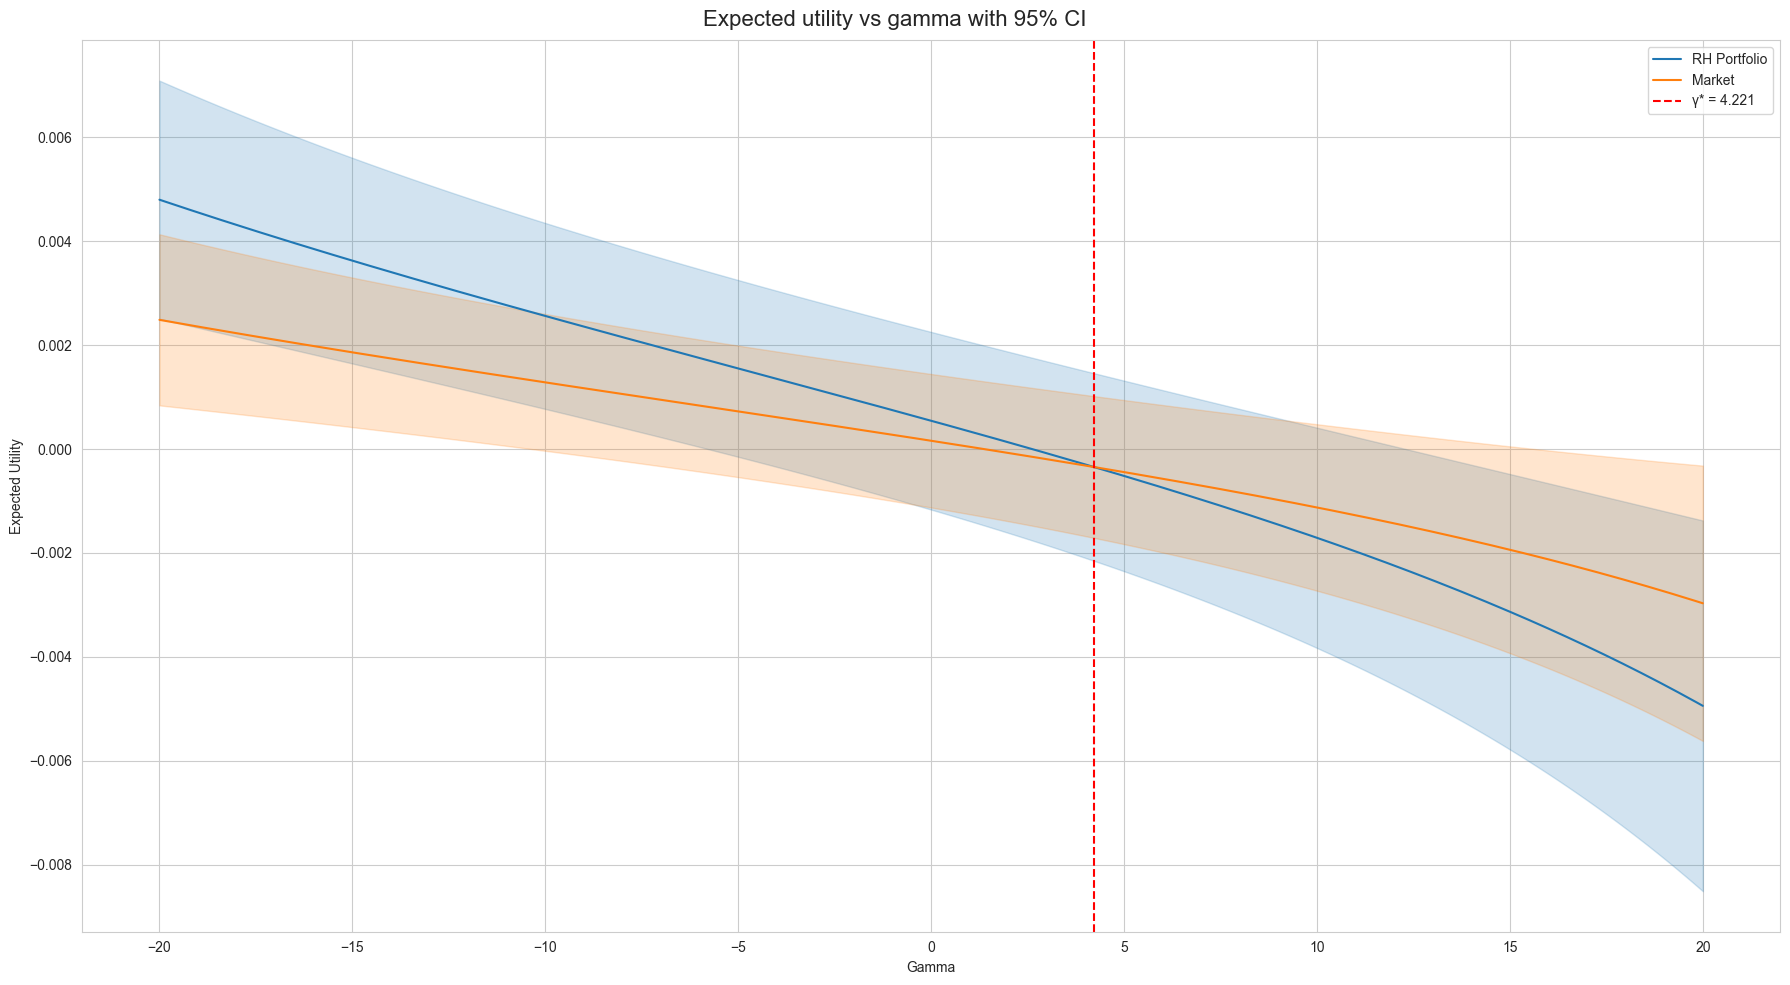
\includegraphics[width=\linewidth]{../images/risk/cutoff_daily.png}
    \caption{Utility for the Robinhood and Market portfolios evaluated over a grid of $\gamma$.}
    \label{fig:cutoff}
\end{figure}

\subsubsection{Augmented Return Sample via All Date-Pairs}
\label{sec:allpairs}
To overcome the limited information in only 539 daily observations, we construct an "all-pairs" dataset that dramatically amplifies our effective sample.  
Specifically, let the trading-day indices in our original series be $1,2,\dots,T$.  
For every ordered pair of dates $(i,j)$ with $1 \le i < j \le T$, we compute the cumulative excess return (net of the risk-free rate) between day $i$ and day $j$ as
\begin{equation}
    R_{i,j}
    \;=\;
    \prod_{k=i+1}^{j}\bigl(1 + r_k - r_{f,k}\bigr),
    \quad
    1 \le i < j \le T,
    \label{eq:allpairs_return}
\end{equation}
where $r_k$ is the portfolio return on day $k$ and $r_{f,k}$ is the daily risk-free rate.  
Using excess returns over the risk-free rate is necessary due to the changes in macroeconomic policy during the time of the sample. 
We treat each multi-day return $R_{i,j}$ as a separate outcome in the investor's distribution of possible holding-period returns, we increase the number of observations from $T$ to $T(T-1)/2$, which reduces sampling variability in our utility-based estimates.  
This "all-pairs" approach preserves the time-ordering of returns while allowing us to evaluate expected utility cutoffs with far greater precision.  

In practice, this results in finding a very low $\gamma^*$ that satisfies equation \ref{gamma_cutoff}, meaning that every investor with a reasonable risk-aversion parameter under CRRA utility would have a greater utility by investing in the market\footnote{
Both the risk-free rate and market returns are downloaded from Kenneth R. French data library \url{https://mba.tuck.dartmouth.edu/pages/faculty/ken.french/data_library.html}}.
In some cases, particularly when ending the sample before the pandemic, the utility curves fitted on the "all-pairs" dataset simply do not intersect for a wide grid of possible risk aversion,
and in fact we find also that in these cases the market stochastically dominates the robinhood portfolio (something which will be analyzed more in depth later).

Performing this exercise for the whole period on the two alternative Robinhood portfolios yields very telling results.
In both instances the cutoff risk aversion as defined in \ref{gamma_cutoff} is negative; 
in particular, the portfolio I constructed has a cutoff risk aversion of -5.437 while the one built using the alternative method we obtain -5.239.
The plot below shows this finding, only extremely risk loving investors would prefer the Robinhood portfolios over a diversified index.  

\begin{figure}[H]
  \centering
  \subfloat[Robinhood Returns Built from Prices]{%
    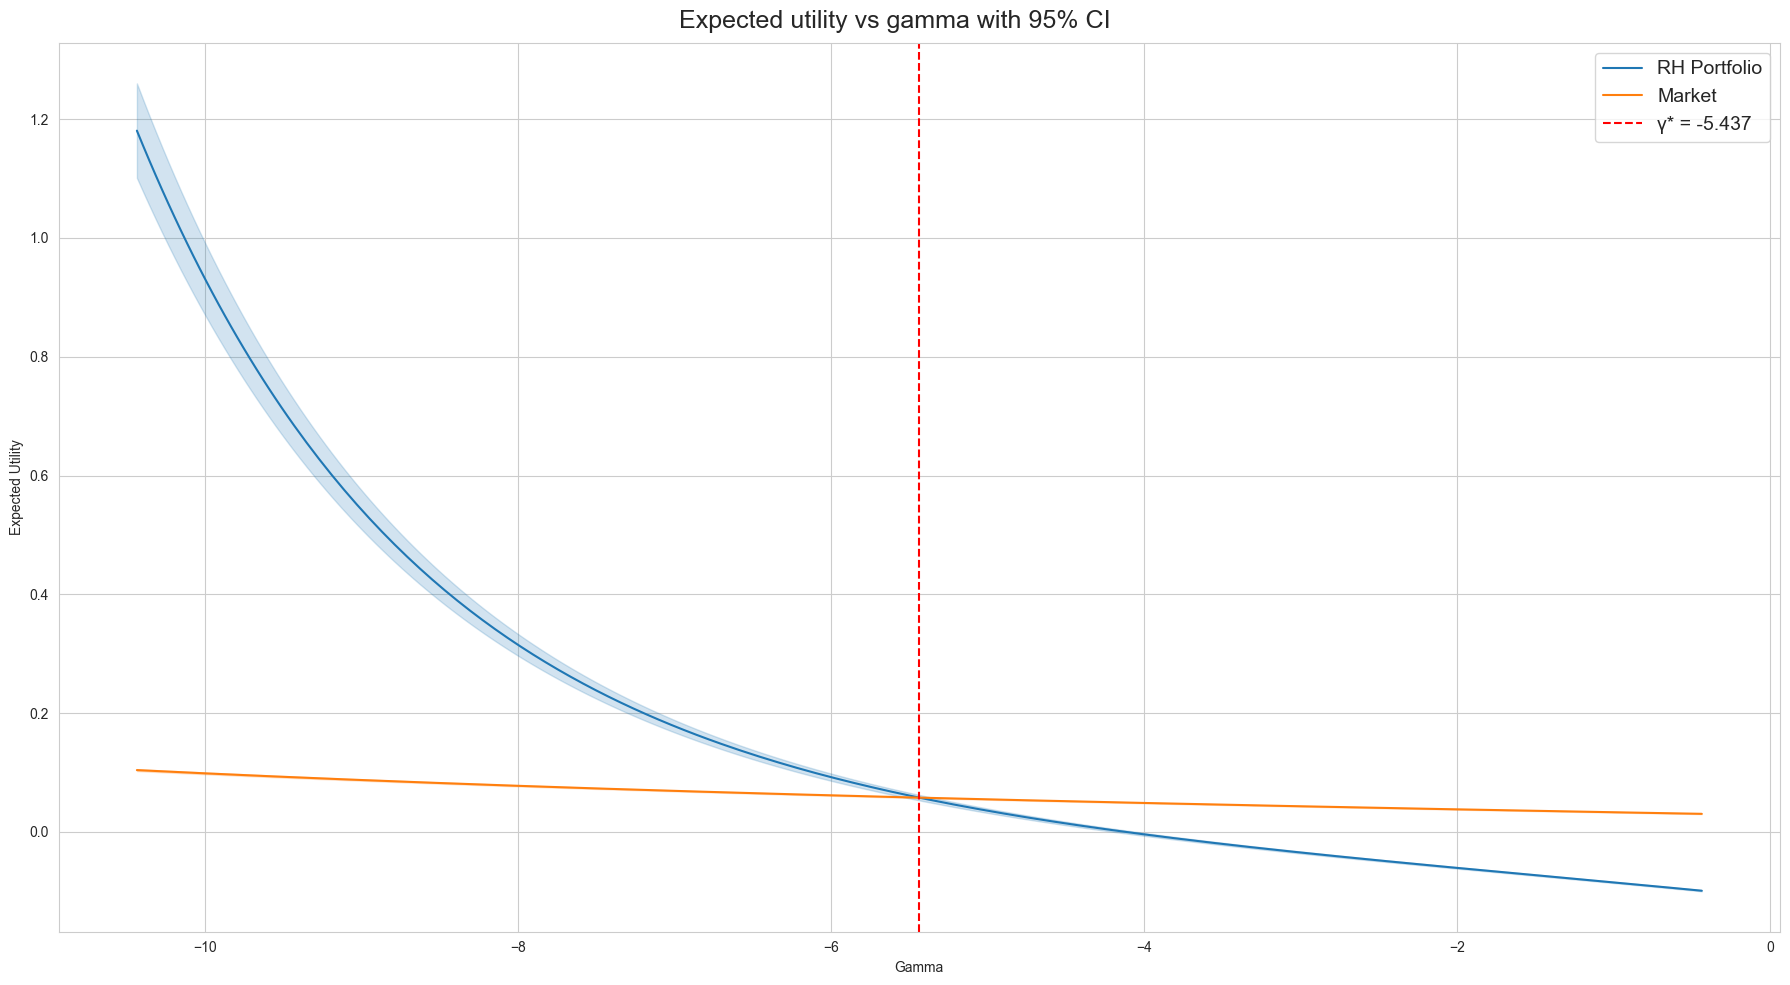
\includegraphics[width=0.48\textwidth]{../images/risk/cutoff_number_all.png}%
    \label{fig:cutoff_number_all}
  }
  \hfill
  \subfloat[Robinhood Returns Built Following Fedyk]{%
    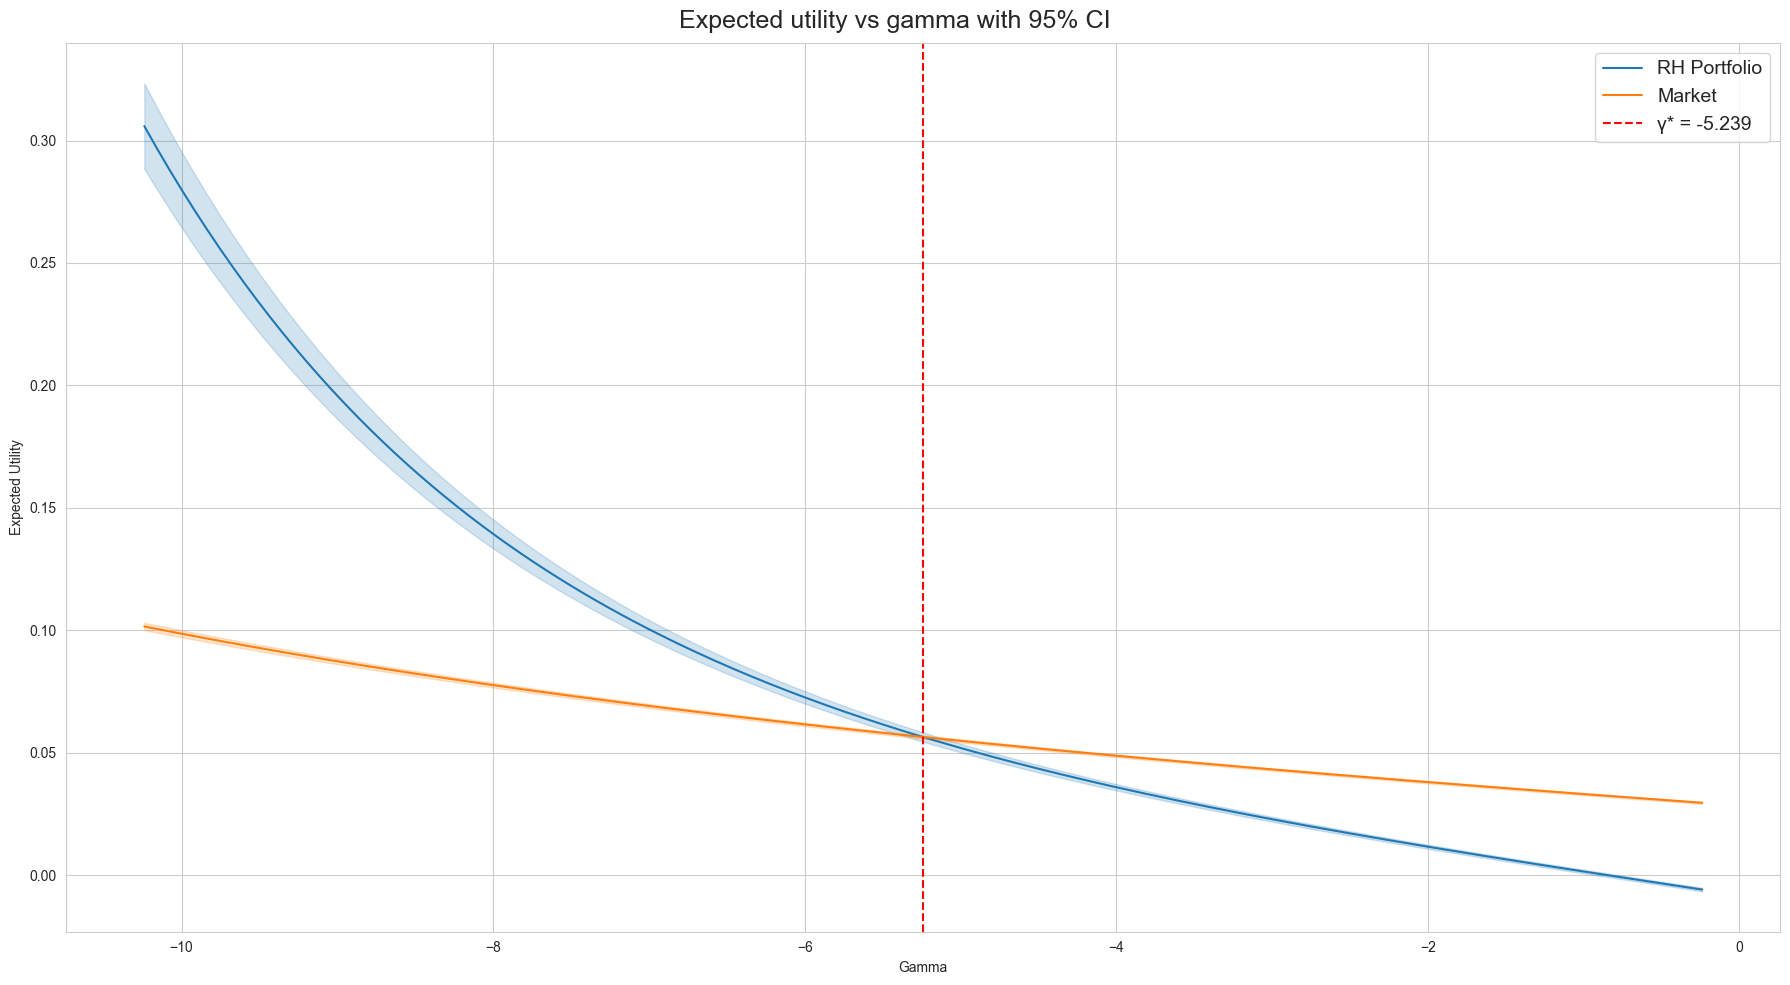
\includegraphics[width=0.48\textwidth]{../images/risk/cutoff_wealth_all.png}%
    \label{fig:cutoff_wealth_all}
  }
  \caption{Expected Utility and Cutoff Risk-aversion for the Robinhood and Market Portfolio.}
  \label{fig:cutoff_all_sidebyside}
\end{figure}

The only case in which $\gamma^*$ is positive is when we compare the Fedyk Portfolio and the World equity ETF as a proxy for the market index, obtaining a value of 1.214.
This implies that weakly risk-averse and risk-loving investors would have a greater utility by investing in this index.
However, if we limit the analysis to the pre-COVID period, the utility of the World ETF strictly dominates for each $\gamma\geq-15.813$, 
highlighting that the former result might indeed be a result of the volatility experienced in early 2020.  

\subsection{Implied Risk Aversion Approach}
\subsubsection{Deriving the Condition}
To address the limitations of our cutoff $\gamma$ approach, we turn to the canonical condition of maximizing expected utility by changing the share of wealth invested in the risky asset.  
In this framework, the agent decides to invest an amount $\alpha$ in the risky asset, his final wealth is therefore:
\begin{equation}
    W_1 = (1-\alpha) W_0 R_f  + \alpha W_0 \tilde R 
    \label{risky_portfolio}
\end{equation}
where $W_0$ is the initial wealth, which we can assume w.l.o.g equal to 1, $R_f$ is the gross return of the risk free asset and $\tilde R$ is the random variable that expresses the returns in the risky asset.

Defining $r=\tilde R - R_f$ we can approximate the CRRA utility of \ref{risky_portfolio} with a second-order taylor expansion around $R_f$:
\begin{equation}
    \mathbb{E}[U(W_1)] \approx R_f^{-\gamma} [\alpha \mathbb{E}[r] - \frac{\gamma}{2}\alpha^2\mathbb{E}[r^2]]
\end{equation} 

The investor chooses its portfolio to maximize the expected utility:
\begin{equation}
    \max_{0 \,\le\, \alpha \,\le\, 1}\; \mathbb{E}[U(W_1)]
    \;\approx\;
    \max_{0 \,\le\, \alpha \,\le\, 1}\;
    R_f^{-\gamma}\Bigl[\alpha\,\mathbb{E}[r]\;-\;\tfrac{\gamma}{2}\,\alpha^2\,\mathbb{E}[r^2]\Bigr]
\end{equation}

which yields the following equation\footnote{
    Derivation:
    $\text{FOC:}\quad
    \frac{\partial}{\partial \alpha}\Bigl\{R_f^{-\gamma}[\alpha\,\mathbb{E}[r]-\tfrac{\gamma}{2}\alpha^2\mathbb{E}[r^2]]\Bigr\}
    =
    R_f^{-\gamma}\bigl(\mathbb{E}[r]-\gamma\,\alpha\,\mathbb{E}[r^2]\bigr)
    \;=\;0$}:
\begin{equation}
    \alpha^*=
    \frac{\mathbb{E}[r]}{\gamma\,\mathbb{E}[r^2]}
\end{equation}

where $\mathbb{E}[r]=\mu-R_f$ and $\mathbb{E}[r^2]=\sigma^2+(\mu-R_f)^2$. 
Since returns are small, $(\mu-R_f)^2\ll\sigma^2$. We derive the following:
\begin{equation}
    \gamma^* = \frac{\mu-R_f}{\alpha \sigma^2}
    \label{gamma_star}
\end{equation}

In our case, both $\alpha$ and $\gamma$ are unknown. 
The variable of interest is $\gamma$, we can therefore use \ref{gamma_star} to compute it for every $\alpha$ in $[0,1]$. 


\subsubsection{Empirical Estimates and Interpretation}
\label{sec:gamma_estimates}
Since we have limited $\alpha$ to be in $[0,1]$ and $\sigma^2 \geq 0$, the implied risk aversion can be negative only if the mean excess returns are negative.

Another relevant point that should be discussed is the choice of not using rolling returns. 
Although they provide a good proxy for assessing the typical return over different horizons and across secruties, 
these return series suffer from autocorellation by construction, implying a very small variance especially at longer horizons.
Therefore, the risk aversion estimates provided by \ref{gamma_star} are unreliable and orders of magnitude greater than acceptable values in asset pricing.
For this reason, we focus or attention on daily, weekly, monthly and three-month returns starting from the first day in the sample. This will avoid the problem with autocorrelation and provide interpretable and useful estimates over different horizons.





\begin{appendices}
\section{Tables}


\begin{table}[ht]
\centering
\caption{Descriptive Statistics for Daily and Rolling Returns}
\begin{adjustbox}{width=\textwidth}
    \begin{tabular}{@{}lllllllll@{}}
    \toprule
    \multicolumn{1}{r}{\textbf{}}       & \multicolumn{1}{r}{\textbf{count}} & \multicolumn{1}{r}{\textbf{mean}} & \multicolumn{1}{r}{\textbf{std}} & \multicolumn{1}{r}{\textbf{min}} & \multicolumn{1}{r}{\textbf{25\%}} & \multicolumn{1}{r}{\textbf{50\%}} & \multicolumn{1}{r}{\textbf{75\%}} & \multicolumn{1}{r}{\textbf{max}} \\ \midrule
    \text{rh\_portfolio}              & 564                                & 0.000719                          & 0.018809                         & -0.132368                        & -0.006164                         & 0.001141                          & 0.009484                          & 0.072851                         \\
    \text{mc}                         & 564                                & 0.000396                          & 0.015470                         & -0.125496                        & -0.003944                         & 0.001012                          & 0.006481                          & 0.086673                         \\
    \text{VOO}                        & 564                                & 0.000438                          & 0.015806                         & -0.124870                        & -0.003874                         & 0.000942                          & 0.006632                          & 0.091087                         \\
    \text{VT}                         & 564                                & 0.000184                          & 0.015092                         & -0.123763                        & -0.004568                         & 0.000842                          & 0.005926                          & 0.087470                         \\
    \text{rh\_portfolio\_1\_return}   & 564                                & 0.000719                          & 0.018809                         & -0.132368                        & -0.006164                         & 0.001141                          & 0.009484                          & 0.072851                         \\
    \text{mc\_1\_return}              & 564                                & 0.000396                          & 0.015470                         & -0.125496                        & -0.003944                         & 0.001012                          & 0.006481                          & 0.086673                         \\
    \text{VOO\_1\_return}             & 564                                & 0.000438                          & 0.015806                         & -0.124870                        & -0.003874                         & 0.000942                          & 0.006632                          & 0.091087                         \\
    \text{VT\_1\_return}              & 564                                & 0.000184                          & 0.015092                         & -0.123763                        & -0.004568                         & 0.000842                          & 0.005926                          & 0.087470                         \\
    \text{rh\_portfolio\_5\_return}   & 564                                & 0.003309                          & 0.041768                         & -0.224427                        & -0.012162                         & 0.004643                          & 0.022078                          & 0.153755                         \\
    \text{mc\_5\_return}              & 564                                & 0.001940                          & 0.031094                         & -0.207508                        & -0.008577                         & 0.004961                          & 0.016049                          & 0.151511                         \\
    \text{VOO\_5\_return}             & 564                                & 0.002152                          & 0.030933                         & -0.204425                        & -0.009377                         & 0.005838                          & 0.016464                          & 0.162820                         \\
    \text{VT\_5\_return}              & 564                                & 0.000864                          & 0.030673                         & -0.214262                        & -0.010938                         & 0.003977                          & 0.014857                          & 0.151788                         \\
    \text{rh\_portfolio\_30\_return}  & 564                                & 0.015173                          & 0.133421                         & -0.482722                        & -0.041325                         & 0.020205                          & 0.051931                          & 0.408751                         \\
    \text{mc\_30\_return}             & 564                                & 0.009890                          & 0.080443                         & -0.401515                        & -0.015223                         & 0.025072                          & 0.046527                          & 0.246006                         \\
    \text{VOO\_30\_return}            & 564                                & 0.011115                          & 0.078031                         & -0.401950                        & -0.011124                         & 0.028635                          & 0.046654                          & 0.252864                         \\
    \text{VT\_30\_return}             & 564                                & 0.003681                          & 0.079260                         & -0.406688                        & -0.020644                         & 0.018305                          & 0.039820                          & 0.224464                         \\
    \text{rh\_portfolio\_60\_return}  & 564                                & 0.010727                          & 0.177731                         & -0.377518                        & -0.066831                         & 0.001284                          & 0.070271                          & 0.641470                         \\
    \text{mc\_60\_return}             & 564                                & 0.016554                          & 0.099118                         & -0.356261                        & -0.013618                         & 0.029848                          & 0.062050                          & 0.338109                         \\
    \text{VOO\_60\_return}            & 564                                & 0.019496                          & 0.095149                         & -0.355392                        & -0.009450                         & 0.033666                          & 0.066970                          & 0.337947                         \\
    \text{VT\_60\_return}             & 564                                & 0.004301                          & 0.101282                         & -0.385941                        & -0.024094                         & 0.012486                          & 0.057122                          & 0.328680                         \\
    \text{rh\_portfolio\_120\_return} & 564                                & -0.014462                         & 0.114741                         & -0.310504                        & -0.098157                         & -0.014206                         & 0.053267                          & 0.370780                         \\
    \text{mc\_120\_return}            & 564                                & 0.017214                          & 0.075478                         & -0.307022                        & -0.031108                         & 0.030972                          & 0.070401                          & 0.218409                         \\
    \text{VOO\_120\_return}           & 564                                & 0.024238                          & 0.074347                         & -0.302877                        & -0.027697                         & 0.034991                          & 0.076471                          & 0.231377                         \\
    \text{VT\_120\_return}            & 564                                & -0.006474                         & 0.077296                         & -0.333294                        & -0.056443                         & 0.008282                          & 0.042280                          & 0.186378                         \\
    \text{rh\_portfolio\_564\_return} & 564                                & -0.011075                         & 0.123340                         & -0.382891                        & -0.055196                         & -0.014086                         & 0.045442                          & 0.405724                         \\
    \text{mc\_564\_return}            & 564                                & 0.071788                          & 0.069591                         & -0.200798                        & 0.033823                          & 0.070623                          & 0.106613                          & 0.224508                         \\
    \text{VOO\_564\_return}           & 564                                & 0.094275                          & 0.071760                         & -0.168586                        & 0.051783                          & 0.090626                          & 0.134336                          & 0.251507                         \\
    \text{VT\_564\_return}            & 564                                & 0.001882                          & 0.063696                         & -0.301083                        & -0.024162                         & 0.014363                          & 0.032343                          & 0.121970                         \\ \bottomrule
    \end{tabular}
\end{adjustbox}
\label{tab:returns_stats}
\end{table}



\begin{table}[ht]
\centering
\caption{Descriptive Statistics for 1-Day and 5-Day Returns, Covering the Whole Period \newline \footnotesize{\textit{Note: Positive returns indicate the percentage of days in which the log returns were greater than zero.}}}
\begin{adjustbox}{width=\textwidth}
\begin{tabular}{@{}clllllllll@{}}
    \toprule
    \multicolumn{1}{r}{}     & \multicolumn{1}{r}{\textbf{count}} & \multicolumn{1}{r}{\textbf{mean}} & \multicolumn{1}{r}{\textbf{std}} & \multicolumn{1}{r}{\textbf{min}} & \multicolumn{1}{r}{\textbf{25\%}} & \multicolumn{1}{r}{\textbf{50\%}} & \multicolumn{1}{r}{\textbf{75\%}} & \multicolumn{1}{r}{\textbf{max}} & \multicolumn{1}{r}{\textbf{positive returns}} \\ \midrule
    rh\_portfolio\_1\_return & 564                                & 0.000719                          & 0.018809                         & -0.132368                        & -0.006164                         & 0.001141                          & 0.009484                          & 0.072851                         & 0.553191                                      \\
    mc\_1\_return            & 564                                & 0.000396                          & 0.015470                         & -0.125496                        & -0.003944                         & 0.001012                          & 0.006481                          & 0.086673                         & 0.558511                                      \\
    VOO\_1\_return           & 564                                & 0.000438                          & 0.015806                         & -0.124870                        & -0.003874                         & 0.000942                          & 0.006632                          & 0.091087                         & 0.563830                                      \\
    VT\_1\_return            & 564                                & 0.000184                          & 0.015092                         & -0.123763                        & -0.004568                         & 0.000842                          & 0.005926                          & 0.087470                         & 0.547872                                      \\
    rh\_portfolio\_5\_return & 560                                & 0.003281                          & 0.041909                         & -0.224427                        & -0.012379                         & 0.004643                          & 0.022098                          & 0.153755                         & 0.598214                                      \\
    mc\_5\_return            & 560                                & 0.001913                          & 0.031198                         & -0.207508                        & -0.008632                         & 0.004961                          & 0.016300                          & 0.151511                         & 0.630357                                      \\
    VOO\_5\_return           & 560                                & 0.002128                          & 0.031036                         & -0.204425                        & -0.009442                         & 0.005838                          & 0.016494                          & 0.162820                         & 0.635714                                      \\
    VT\_5\_return            & 560                                & 0.000839                          & 0.030779                         & -0.214262                        & -0.011044                         & 0.003977                          & 0.014911                          & 0.151788                         & 0.583929                                      \\ \bottomrule
\end{tabular}
\end{adjustbox}
\label{tab:st_returns_stats_all}
\end{table}

\begin{table}[ht]
\centering
\caption{Descriptive Statistics for 1-Day and 5-Day Returns, up to February 3rd 2020
\newline \footnotesize{\textit{Note: Positive returns indicate the percentage of days in which the log returns were greater than zero.}}}
\begin{adjustbox}{width=\textwidth}
\begin{tabular}{@{}clllllllll@{}}
    \toprule
    \multicolumn{1}{r}{\textbf{}}     & \multicolumn{1}{r}{\textbf{count}} & \multicolumn{1}{r}{\textbf{mean}} & \multicolumn{1}{r}{\textbf{std}} & \multicolumn{1}{r}{\textbf{min}} & \multicolumn{1}{r}{\textbf{25\%}} & \multicolumn{1}{r}{\textbf{50\%}} & \multicolumn{1}{r}{\textbf{75\%}} & \multicolumn{1}{r}{\textbf{max}} & \multicolumn{1}{r}{\textbf{positive returns}} \\ \midrule
    \text{rh\_portfolio\_1\_return} & 430                                & 0.000115                          & 0.013490                         & -0.050597                        & -0.005461                         & 0.000809                          & 0.007377                          & 0.068808                         & 0.537209                                      \\
    \text{mc\_1\_return}            & 430                                & 0.000419                          & 0.008745                         & -0.032113                        & -0.003126                         & 0.000804                          & 0.005285                          & 0.045916                         & 0.553488                                      \\
    \text{VOO\_1\_return}           & 430                                & 0.000485                          & 0.008928                         & -0.032828                        & -0.003066                         & 0.000757                          & 0.005096                          & 0.049350                         & 0.558140                                      \\
    \text{VT\_1\_return}            & 430                                & 0.000198                          & 0.008361                         & -0.031068                        & -0.003794                         & 0.000716                          & 0.004853                          & 0.036545                         & 0.546512                                      \\
    \text{rh\_portfolio\_5\_return} & 426                                & 0.000259                          & 0.026549                         & -0.105948                        & -0.013623                         & 0.002922                          & 0.014899                          & 0.088194                         & 0.570423                                      \\
    \text{mc\_5\_return}            & 426                                & 0.002091                          & 0.019395                         & -0.075729                        & -0.008188                         & 0.004110                          & 0.014121                          & 0.063052                         & 0.624413                                      \\
    \text{VOO\_5\_return}           & 426                                & 0.002442                          & 0.019790                         & -0.081061                        & -0.008308                         & 0.004981                          & 0.014449                          & 0.067072                         & 0.636150                                      \\
    \text{VT\_5\_return}            & 426                                & 0.001031                          & 0.018612                         & -0.066412                        & -0.010824                         & 0.002804                          & 0.013208                          & 0.060003                         & 0.565728                                      \\ \bottomrule
\end{tabular}    
\end{adjustbox}
\label{tab:st_returns_stats_before}
\end{table}


\newpage
\section{Handling Missing Data}
\label{sec:data}
The original Robinhood dataset contains missing values for 3,331 securities, primarily in the earlier periods. 
This means that these securities don't have information for a certain date.
   
To ensure consistency we adopt a similar method as \cite{Fedyk2024}. Their Robinhood portfolio is constructed using the available securities on a daily basis, 
hence securities with missing values are simply not taken into account for the day. Moreover we drop all securities that they have defined as problematic in the appendix.

Since our CRSP dataset is also a bit different from the one they use, we drop entirely securities that have more than one entry per day.


\end{appendices}

% References Section
\bibliographystyle{apalike}  % Use APA-style references (or another style)
\bibliography{references}  % Load references.bib


\end{document}